\Problem
{گام سوم}
{
سوالات پرسیده شده در متن را با استفاده از کد متلب پاسح می‌دهیم.

\begin{figure}[H]
    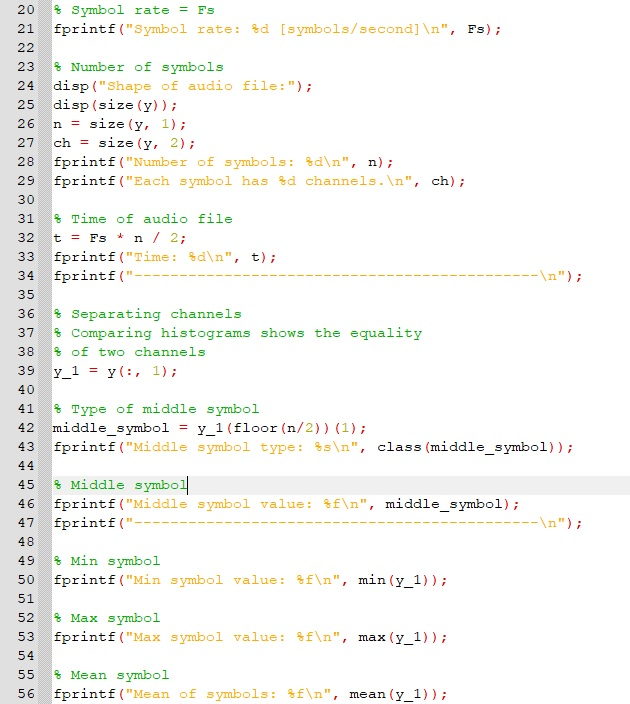
\includegraphics[width=15cm]{Images/step_3_code.jpg}
    \centering
    \caption{کد مربوط به پرینت مولفه‌های گام دوم}
\end{figure}

خروجی این قسمت به صورت زیر است:
\begin{latin}
\newline
Symbol rate: 22050 [symbols/second]
\newline
Shape of audio file: 87462       1
\newline
Number of symbols: 87462
\newline
Each symbol has 1 channels.
\newline
Time: 3.96653
\newline
---------------------------------------------
\newline
Middle symbol type: double
\newline
Middle symbol value: 0.008942
\newline
---------------------------------------------
\newline
Min symbol value: -0.928558
\newline
Max symbol value: 0.978363
\newline
Mean of symbols: -0.000313
\end{latin}

به تعداد \lr{87462} سمبل داریم که هر یک از جنس 
\lr{double} است که دقت آن تا 7 رقم اعشار هست. برای ذخیره سازی این فرمت نیاز به 8 بایت داریم.

نرخ سمبل در ثانیه برابر \lr{22050} شده است. یعنی در هر ثانیه آن تعداد سمبل داریم.

مقادیر هر سمبل میان عدد \lr{-1} تا \lr{1} است.

از تقسیم تعداد سمبل در نرخ سمبل بر ثانیه می‌توانیم به زمان فایل صوتی برسیم. که این عدد تقریبا نزدیک 4 شده است.

طبق قضیه نایکویست با توجه به اینکه نرخ نمونه برداری بزرگتر از 2 برابر بیشینه فرکانس بوده است، می‌توان از سیگنال ثانویه به سیگنال اولیه رسید. و پدیده آلیاسینگ نداریم به همین دلیل است که صوت گسستگی نداریم.

همچنین فرکانس شنوایی انسان از نرخ این صوت پایین تر است و ما آن را پیوسته می‌شنویم. در هنگام مشاهده فیلم نیز همین اتفاق می‌افتد زیرا چشم انسان نهایتن تا \lr{24} فریم بر ثانیه را می‌تواند تشخیص دهد و اگر فریم ریت این فیلم بالاتر از این نرخ باشد ما آن را پیوسته مشاهده می‌کنیم.
}